\documentclass[11pt,a4paper]{article}

\usepackage{../ve401}
\usepackage{tikz}
\usetikzlibrary{arrows.meta}
\usetikzlibrary{patterns}

\author{Group 37}
\semester{Spring}
\year{2019}
\subtitle{Assignment}
\subtitlenumber{2}
\blockinfo{
	\bigskip
	\begin{center}
		\textbf{Group members}
	\end{center}
	\begin{itemize}\itemsep .25cm
		\item \href{mailto:hcm_9809@sjtu.edu.cn}{Chenmin Hou} (517370910248)
		\item \href{mailto:liuyh615@126.com}{Yihao Liu} (515370910207)
		\item \href{mailto:lyz0123@sjtu.edu.cn}{Yuzhou Li} (517021910922)
	\end{itemize}
}

\begin{document}

\maketitle

\subsection{Drawing until First Success in the Hypergeometric Setting}

\begin{enumerate}[label=\roman*)]
\item
Let $H[n]$ be the unit step function, such that 
$$H[n]=\left\{\begin{aligned}
0&\quad n<0\\1&\quad n\geqslant 0
\end{aligned}\right..$$
Since ${\rm ran}\ X\subset \mathbb{N}$,
$$E[X]=\sum_{x\in N}x\cdot f_X(x)=\sum_{x=1}^\infty x\cdot P[X=x]=\sum_{x=0}^\infty x\cdot P[X=x].$$
And
\begin{align*}
\sum_{x=0}^\infty P[X>x]
&=\sum_{x=0}^\infty\sum_{y=x+1}^\infty P[X=y]\\
&=\sum_{x=0}^\infty\sum_{y=0}^\infty P[X=y]H[y-x-1]\\
&=\sum_{y=0}^\infty P[X=y]\sum_{x=0}^\infty H[y-x-1]\\
&=\sum_{y=0}^\infty P[X=y]\cdot y\\
&=E[X].
\end{align*}
\item
Let $x$ be the number of balls drawn, $x\in [0,N-r+1]\cap\mathbb{N}$
$$P[X>x]=\frac{\binom{r}{0}\binom{N-r}{x-0}}{\binom{N}{x}}=\frac{\binom{N-r}{x}}{\binom{N}{x}}=\frac{\frac{(N-r)!}{x!(N-r-x)!}}{\frac{N!}{x!(N-x)!}}=\frac{(N-r)!(N-x)!}{N!(N-r-x)!}.$$
According to i),
$$E[X]=\sum_{x=0}^\infty P[X>x]=\frac{(N-r)!}{N!}\sum_{x=0}^{N-r} \frac{(N-x)!}{(N-r-x)!}=\frac{(N-r)!r!}{N!}\sum_{x=0}^{N-r}\binom{N-x}{r}.$$
Let $k=N-r-x$, $b=N-r$,
\begin{align*}
E[X]&=\frac{(N-r)!r!}{N!}\sum_{k=0}^{N-r}\binom{r+k}{r}
=\frac{(N-r)!r!}{N!}\sum_{k=0}^{b}\binom{N-b+k}{N-b}\\
&=\frac{(N-r)!r!}{N!}\binom{N+1}{N-b+1}
=\frac{(N-r)!r!}{N!}\cdot\frac{(N+1)!}{(r+1)!(N-r)!}\\
&=\frac{N+1}{r+1}.
\end{align*}
\end{enumerate}

\subsection{Density of the Poisson Approximation}

Suppose $$p_x(t)=\frac{(\lambda t)^xe^{-\lambda t}}{x!}.$$
When $x=0$,
$$p_0'=-\lambda p_0\Longrightarrow p_0(t)=Ce^{-\lambda t}.$$
Since the probability of $x=0$ arrivals at time $t=0$ is 1, we can obtain $p_0(0)=1$, then
$$p_0(t)=e^{-\lambda t},$$
which satisfy the formula of $p_x(t)$.

When $x=x+1$,
$$p_{x+1}'(t)+\lambda p_{x+1}(t)=\lambda p_x(t)=\frac{\lambda(\lambda t)^xe^{-\lambda t}}{x!}.$$
Let $p_{x+1}(t)=u(t)e^{-\int\lambda dt}=u(t)e^{-\lambda t}$,
$$u'(t)=\frac{\frac{\lambda(\lambda t)^xe^{-\lambda t}}{x!}}{e^{-\int\lambda dt}}=\frac{\lambda(\lambda t)^x}{x!}.$$
$$p_{x+1}(t)=e^{-\lambda t}\int u'(t)dt=e^{-\lambda t}\int\frac{\lambda(\lambda t)^x}{x!}dt=e^{-\lambda t}\frac{1}{(x+1)\lambda}\frac{\lambda(\lambda t)^{x+1}}{x!}=\frac{(\lambda t)^{x+1}                                                                                                                                                                                                                              e^{-\lambda t}}{(x+1)!},$$
which satisfy the formula of $p_x(t)$.

So it is proved by induction.

\subsection{Poisson Approximation to the Binomial Distribution}

$$f(x)=\binom{n}{x}p^x(1-p)^{n-x}=\frac{n!}{x!(n-x)!}\left(\frac{k}{n}\right)^x\left(1-\frac{k}{n}\right)^{n-x}.$$
$$\lim_{n\to\infty}\frac{n!}{(n-x)!}=\lim_{n\to\infty}\prod_{k=0}^{x-1}(n-k)=n^x.$$
$$\lim_{n\to\infty}n\ln\left(1-\frac{k}{n}\right)=\lim_{n\to\infty}\frac{\ln\left(1-\frac{k}{n}\right)}{\frac{1}{n}}=\lim_{n\to\infty}\frac{\frac{1}{1-\frac{k}{n}}\cdot\frac{k}{n^2}}{-\frac{1}{n^2}}=-k,$$
$$\lim_{n\to\infty}\left(1-\frac{k}{n}\right)^{n-x}=\lim_{n\to\infty}\left(1-\frac{k}{n}\right)^n=\exp\left[{\lim_{n\to\infty}n\ln\left(1-\frac{k}{n}\right)}\right]=e^{-k}.$$
So $$\lim_{n\to\infty}f(x)=\frac{n!k^x}{x!(n-x)!n^x}\left(1-\frac{k}{n}\right)^{n-x}=\frac{k^xe^{-k}}{x!}.$$

\subsection{Maxwell-Boltzmann Statistics}
Let $$k_0=-\frac{m}{2kT},\quad k_1=\left(\frac{2}{\pi}\right)^{1/2}\left(\frac{m}{kT}\right)^{3/2},$$
when $v>0$,
$$f_V(v)=k_1v^2e^{-k_0v^2/2}.$$
\begin{enumerate}[label=\roman*)]
\item
\begin{align*}
{\rm Mean}[V]=E[V]&=\int_0^\infty v\cdot f_V(v)dv=k_1\int_0^\infty v^3e^{k_0v^2}dv\\
&=\frac{k_1}{2k_0}\int_1^0 v^2d(e^{k_0v^2})\Longleftarrow k_0<0\\
&=\frac{k_1}{2k_0}\int_1^0 \frac{\ln(e^{k_0v^2})}{k_0}d(e^{k_0v^2})\Longleftarrow u=e^{k_0v^2}\\
&=\frac{k_1}{2k_0^2}\cdot u(\ln u-1)\bigg|_1^0=\frac{k_1}{2k_0^2}\\
&=2\left(\frac{2}{\pi}\right)^{1/2}\left(\frac{m}{kT}\right)^{-1/2}
\end{align*}
Let
$$I(k_0)=\int_0^\infty e^{k_0v^2}dv=\int_0^\infty e^{k_0u^2}du,$$
then
\begin{align*}
I^2(k_0)&=\int_0^\infty\int_0^\infty e^{k_0(u^2+v^2)}dudv\\
&=\int_0^{\pi/2}\int_0^\infty re^{k_0r^2}drd\theta\\
&=\int_0^{\pi/2}\int_1^0 \frac{1}{2k_0} d(e^{k_0r^2})d\theta\Longleftarrow k_0<0\\
&=\frac{1}{2k_0}\int_0^{\pi/2}u\bigg|_1^0d\theta\Longleftarrow u=e^{k_0v^2}\\
&=\frac{1}{2k_0}\int_0^{\pi/2}-1d\theta=-\frac{\pi}{4k_0},
\end{align*}
$$I(k_0)=\sqrt{-\frac{\pi}{4k_0}}=\frac{\sqrt{\pi}}{2}(-k_0)^{-1/2}.$$
Differentiate on $k_0$, we can get
$$I'(k_0)=\int_0^\infty v^2e^{k_0v^2}dv=\frac{\sqrt{\pi}}{4}(-k_0)^{-3/2},$$
$$I''(k_0)=\int_0^\infty v^4e^{k_0v^2}dv=\frac{3\sqrt{\pi}}{8}(-k_0)^{-5/2}.$$
\begin{align*}
E[V^2]&=\int_0^\infty v^2\cdot f_V(v)dv=k_1\int_0^\infty v^4e^{k_0v^2}dv\\
&=k_1\frac{3\sqrt{\pi}}{8}(-k_0)^{-5/2}\\
&=\left(\frac{2}{\pi}\right)^{1/2}\left(\frac{m}{kT}\right)^{3/2}\frac{3\sqrt{\pi}}{8}\left(\frac{m}{2kT}\right)^{-5/2}\\
&=\frac{3kT}{m}.
\end{align*}
$${\rm Var}[X]=E[V^2]-(E[V])^2=\frac{3kT}{m}-\frac{8}{\pi}\frac{kT}{m}=\left(3-\frac{8}{\pi}\right)\frac{kT}{m}.$$
\item
$${\rm Mean}[mV^2/2]=E[mV^2/2]=\frac{m}{2}E[V^2]=\frac{3kT}{2}.$$
\item
Let $\varphi(V)=mV^2/2$, when $v>0$, $\varphi:\mathbb{R}^+\to\mathbb{R}^+$ is strictly monotonic and differentiable. According to Theorem 1.3.13,
$$f_E(E)=f_v(\varphi^{-1}(E))\cdot\left|\frac{d\varphi^{-1}(E)}{dE}\right|,$$
$$\varphi^{-1}(E)=\sqrt{\frac{2E}{m}}=\sqrt{\frac{2}{m}}E^{1/2},$$
$$\frac{d\varphi^{-1}(E)}{dE}=\sqrt{\frac{1}{2m}}E^{-1/2}=\sqrt{\frac{1}{2mE}},$$
When $v>0$,
$$f_E(E)=\left(\frac{2}{\pi}\right)^{1/2}\left(\frac{m}{kT}\right)^{3/2}\frac{2E}{m}e^{-\frac{m}{kT}\frac{2E}{m}/2}\sqrt{\frac{1}{2mE}},$$
and when $v\leqslant 0$, $f_E(E)=0$.

In conclusion,
$$f_E(E)=\left\{\begin{aligned}
&\left(\frac{2}{\pi}\right)^{1/2}\left(\frac{1}{kT}\right)^{3/2}e^{-\frac{E}{kT}}\sqrt{2E}&\quad E>0\\
&0&\quad E\leqslant0
\end{aligned}\right..$$
\end{enumerate}

\subsection{Half-Integer Values of the Gamma Function}

$$\Gamma\left(\frac{2n+1}{2}\right)=\int_0^\infty z^{\frac{2n-1}{2}}e^{-z}dz=\int_0^\infty z^{\frac{2n-1}{2}}e^{-z}d(\sqrt{z})=2\int_0^\infty\sqrt{z}^{2n}e^{-\sqrt{z}^2}d(\sqrt{z})=2\int_0^\infty u^{2n}e^{-u^2}du.$$
According to the result of Gaussian Integral derived in Exercise 2.4,
$$I(a)=2\int_0^\infty e^{au^2}du=2\sqrt{\frac{\pi}{-4a}}=\pi(-a)^{-1/2},$$
$$\frac{d^nI(a)}{da^n}=2\int_0^\infty u^{2n}e^{au^2}du=\sqrt{\pi}(-a)^{-1/2-n}\prod_{k=1}^n\frac{2k-1}{2}.$$
When $a=-1$,
$$\Gamma\left(\frac{2n+1}{2}\right)=2\int_0^\infty u^{2n}e^{-u^2}du=\sqrt{\pi}\prod_{k=1}^n\frac{2k-1}{2}=\frac{\sqrt{\pi}(2n-1)!!}{2^n}.$$

\subsection{Finding Probabilities with the Normal Distribution}

\begin{enumerate}[label=\roman*)]
\item
$$P[X<6250]=P\left[\frac{X-\mu}{\sigma}<\frac{6250-6000}{100}\right]=P[Z<2.5]=\Phi(2.5)\approx0.9938.$$
\item
\begin{align*}
P[5800\leqslant X\leqslant 5900]&=P\left[\frac{5800-6000}{100}\leqslant\frac{X-\mu}{\sigma}\leqslant\frac{5900-6000}{100}\right]\\
&=P[-2\leqslant Z\leqslant -1]\\
&=\Phi(-1)-\Phi(-2)\\
&\approx0.1587-0.0228=0.1359.
\end{align*}
\item
When $x_0$ is exceeded by 95\% of the samples,
$$P[X<x_0]=P\left[\frac{X-\mu}{\sigma}<\frac{x_0-6000}{100}\right]=P[Z<0.01x_0-60]=\Phi(0.01x_0-60)\leqslant 0.05,$$
$$0.01x_0-60\leqslant\Phi^{-1}(0.95)\approx-1.65,$$
$$x_0\lessapprox5835{\rm~kg/cm^3}.$$
\end{enumerate}

\subsection{Continuous Uniform Distribution}

\begin{enumerate}[label=\roman*)]
\item
From the definition of $f(x)$, we know $f_X(x)\geqslant0$ for all $x\in\mathbb{R}$, and
$$\int_{-\infty}^\infty f_X(x)dx=\int_a^b\frac{1}{b-a}dx=1,$$
so this is a density for a continuous random variable.
\item~
\begin{center}
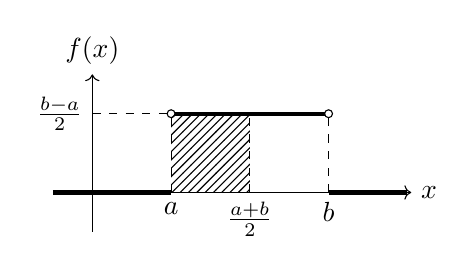
\begin{tikzpicture}
\draw[->] (-0.5,0) -- (4.05,0) node[right] {$x$};
\draw[->] (0,-0.5) -- (0,1.5) node[above] {$f(x)$};
\draw[ultra thick] (-0.5,0) -- (1,0) (3,0) -- (4,0)  (1,1) -- (3,1);
\draw[fill=white] (1,1) circle (0.05) (3,1) circle (0.05);
\draw (1,0) node[below] {$a$};
\draw (2,0) node[below] {$\frac{a+b}{2}$};
\draw (3,0) node[below] {$b$};
\draw (0,1) node[left] {$\frac{b-a}{2}$};
\draw[dashed] (1,0) -- (1,1) (2,0) -- (2,1) (3,0) -- (3,1) (0,1) -- (1,1);
\fill[pattern=north east lines] (1,0) rectangle (2,1);
\end{tikzpicture}
\end{center}
\item
$$P\left[\frac{a+b}{2}\right]=\int_{-\infty}^{(a+b)/2}f_X(x)dx=\int_a^{(a+b)/2}\frac{1}{b-a}dx=\frac{1}{2}.$$
\item
$$P[c\leqslant X\leqslant d]=\int_c^df_X(x)dx=\int_c^d\frac{1}{b-a}dx=\frac{d-c}{b-a},$$
$$P[e\leqslant X\leqslant f]=\int_e^ff_X(x)dx=\int_e^f\frac{1}{b-a}dx=\frac{f-e}{b-a}.$$
Since $d-c=f-e$, we can simply get
$$P[c\leqslant X\leqslant d]=P[e\leqslant X\leqslant f].$$
\item
$$F_X(x)=P[X\leqslant x]=\int_{-\infty}^xf_X(y)dy=\int_{-\infty}^x\frac{1}{b-a}dy,$$
$$F_X(x)=\left\{\begin{aligned}
&0&\quad x\leqslant a\\
&\frac{x-a}{b-a}&\quad a<x<b\\
&1&\quad x\geqslant b
\end{aligned}\right..$$
\item
$$E[X]=\int_{-\infty}^\infty xf_X(x)dx=\int_a^b\frac{x}{b-a}dx=\frac{1}{b-a}\cdot\frac{1}{2}x^2\bigg|_a^b=\frac{a+b}{2}.$$
$$E[X^2]=\int_{-\infty}^\infty x^2f_X(x)dx=\int_a^b\frac{x^2}{b-a}dx=\frac{1}{b-a}\cdot\frac{1}{3}x^3\bigg|_a^b=\frac{a^2+ab+b^2}{3}.$$
$${\rm Var}[X]=E[X^2]-(E[X])^2=\frac{a^2+ab+b^2}{3}-\frac{(a+b)^2}{4}=\frac{(b-a)^2}{12}.$$
\end{enumerate}

\subsection{A Tricky Question involving the Binomial Distribution}

\begin{enumerate}[label=\roman*)]
\item
Let $X$ be the number of errors in a random sample of 50 pages, then
$$P[X>0]=1-P[X=0]=1-\left(\frac{150}{200}\right)^5=\frac{781}{1024}.$$
\item
Let $k$ be the random sample size to assure that at least three errors will be found with 90\% probability, then
$$n=5,\quad p=\frac{k}{200}.$$
$$P[X\leqslant 2]\approx\Phi\left(\frac{2+1/2-np}{\sqrt{np(1-p)}}\right)=\Phi\left(\frac{2+1/2-k/40}{\sqrt{k/40(1-k/200)}}\right)\leqslant0.1.$$
$$\frac{2+1/2-k/40}{\sqrt{k/40(1-k/200)}}\leqslant\Phi^{-1}(0.1)=-1.28.$$
$$(2.5-k/40)^2\geqslant1.28^2\cdot k/40(1-k/200),\quad 2.5-k/40\leqslant 0.$$
$$k\gtrapprox 149.68.$$
So the sample size should be at least 150.
\end{enumerate}

\subsection{Reliability of a System}
\begin{enumerate}[label=\roman*)]
\item 
$$R_1(t)=\exp\left[-\int_0^t\alpha_1\beta_1 x^{\beta_1-1}dx\right]=e^{-\alpha_1 t^{\beta_1}},$$
$$R_2(t)=\exp\left[-\int_0^t\beta_2 dx\right]=e^{-\beta_2 t},$$
$$R_s(t)=R_1(t)R_2(t)=e^{-\alpha_1t^{\beta_1}-\beta_2 t}.$$
$$R_s(2500)=e^{-0.006\cdot2500^{0.5}-1/25000\cdot2500}=e^{-0.4}\approx0.670.$$
\item
$$P[t<2000]=1-R_s(2000)=1-e^{-0.006\cdot2000^{0.5}-1/25000\cdot2000}\approx0.294.$$
\item
$$R_p(t)=1-(1-R_1(t))(1-R_2(t))=1-(1-e^{-\alpha_1 t^{\beta_1}})(1-e^{-\beta_2 t}).$$
$$R_p(2500)=1-(1-e^{-0.006\cdot2500^{0.5}})(1-e^{-1/25000\cdot2500})=e\approx0.975.$$
\end{enumerate}

\end{document}


